
\captionsetup[figure]{labelfont={sc},labelformat={default},labelsep=period,name={Figure}}

%%%%%%%%%%%%%%%%%%%%%%%%%%%%%%%%%%%%%%%%%%%%%%%%%%%%%%%%%%%%%%%%%%%%%%%%%%%%%%%%
%%%%%%%%%%%%%%%%%%%%%%%%%%%%%%%%%%%%%%%%%%%%%%%%%%%%%%%%%%%%%%%%%%%%%%%%%%%%%%%%
%% WORKFLOW FIGURE
%%%%%%%%%%%%%%%%%%%%%%%%%%%%%%%%%%%%%%%%%%%%%%%%%%%%%%%%%%%%%%%%%%%%%%%%%%%%%%%%
%%%%%%%%%%%%%%%%%%%%%%%%%%%%%%%%%%%%%%%%%%%%%%%%%%%%%%%%%%%%%%%%%%%%%%%%%%%%%%%%


\begin{figure}[!h]
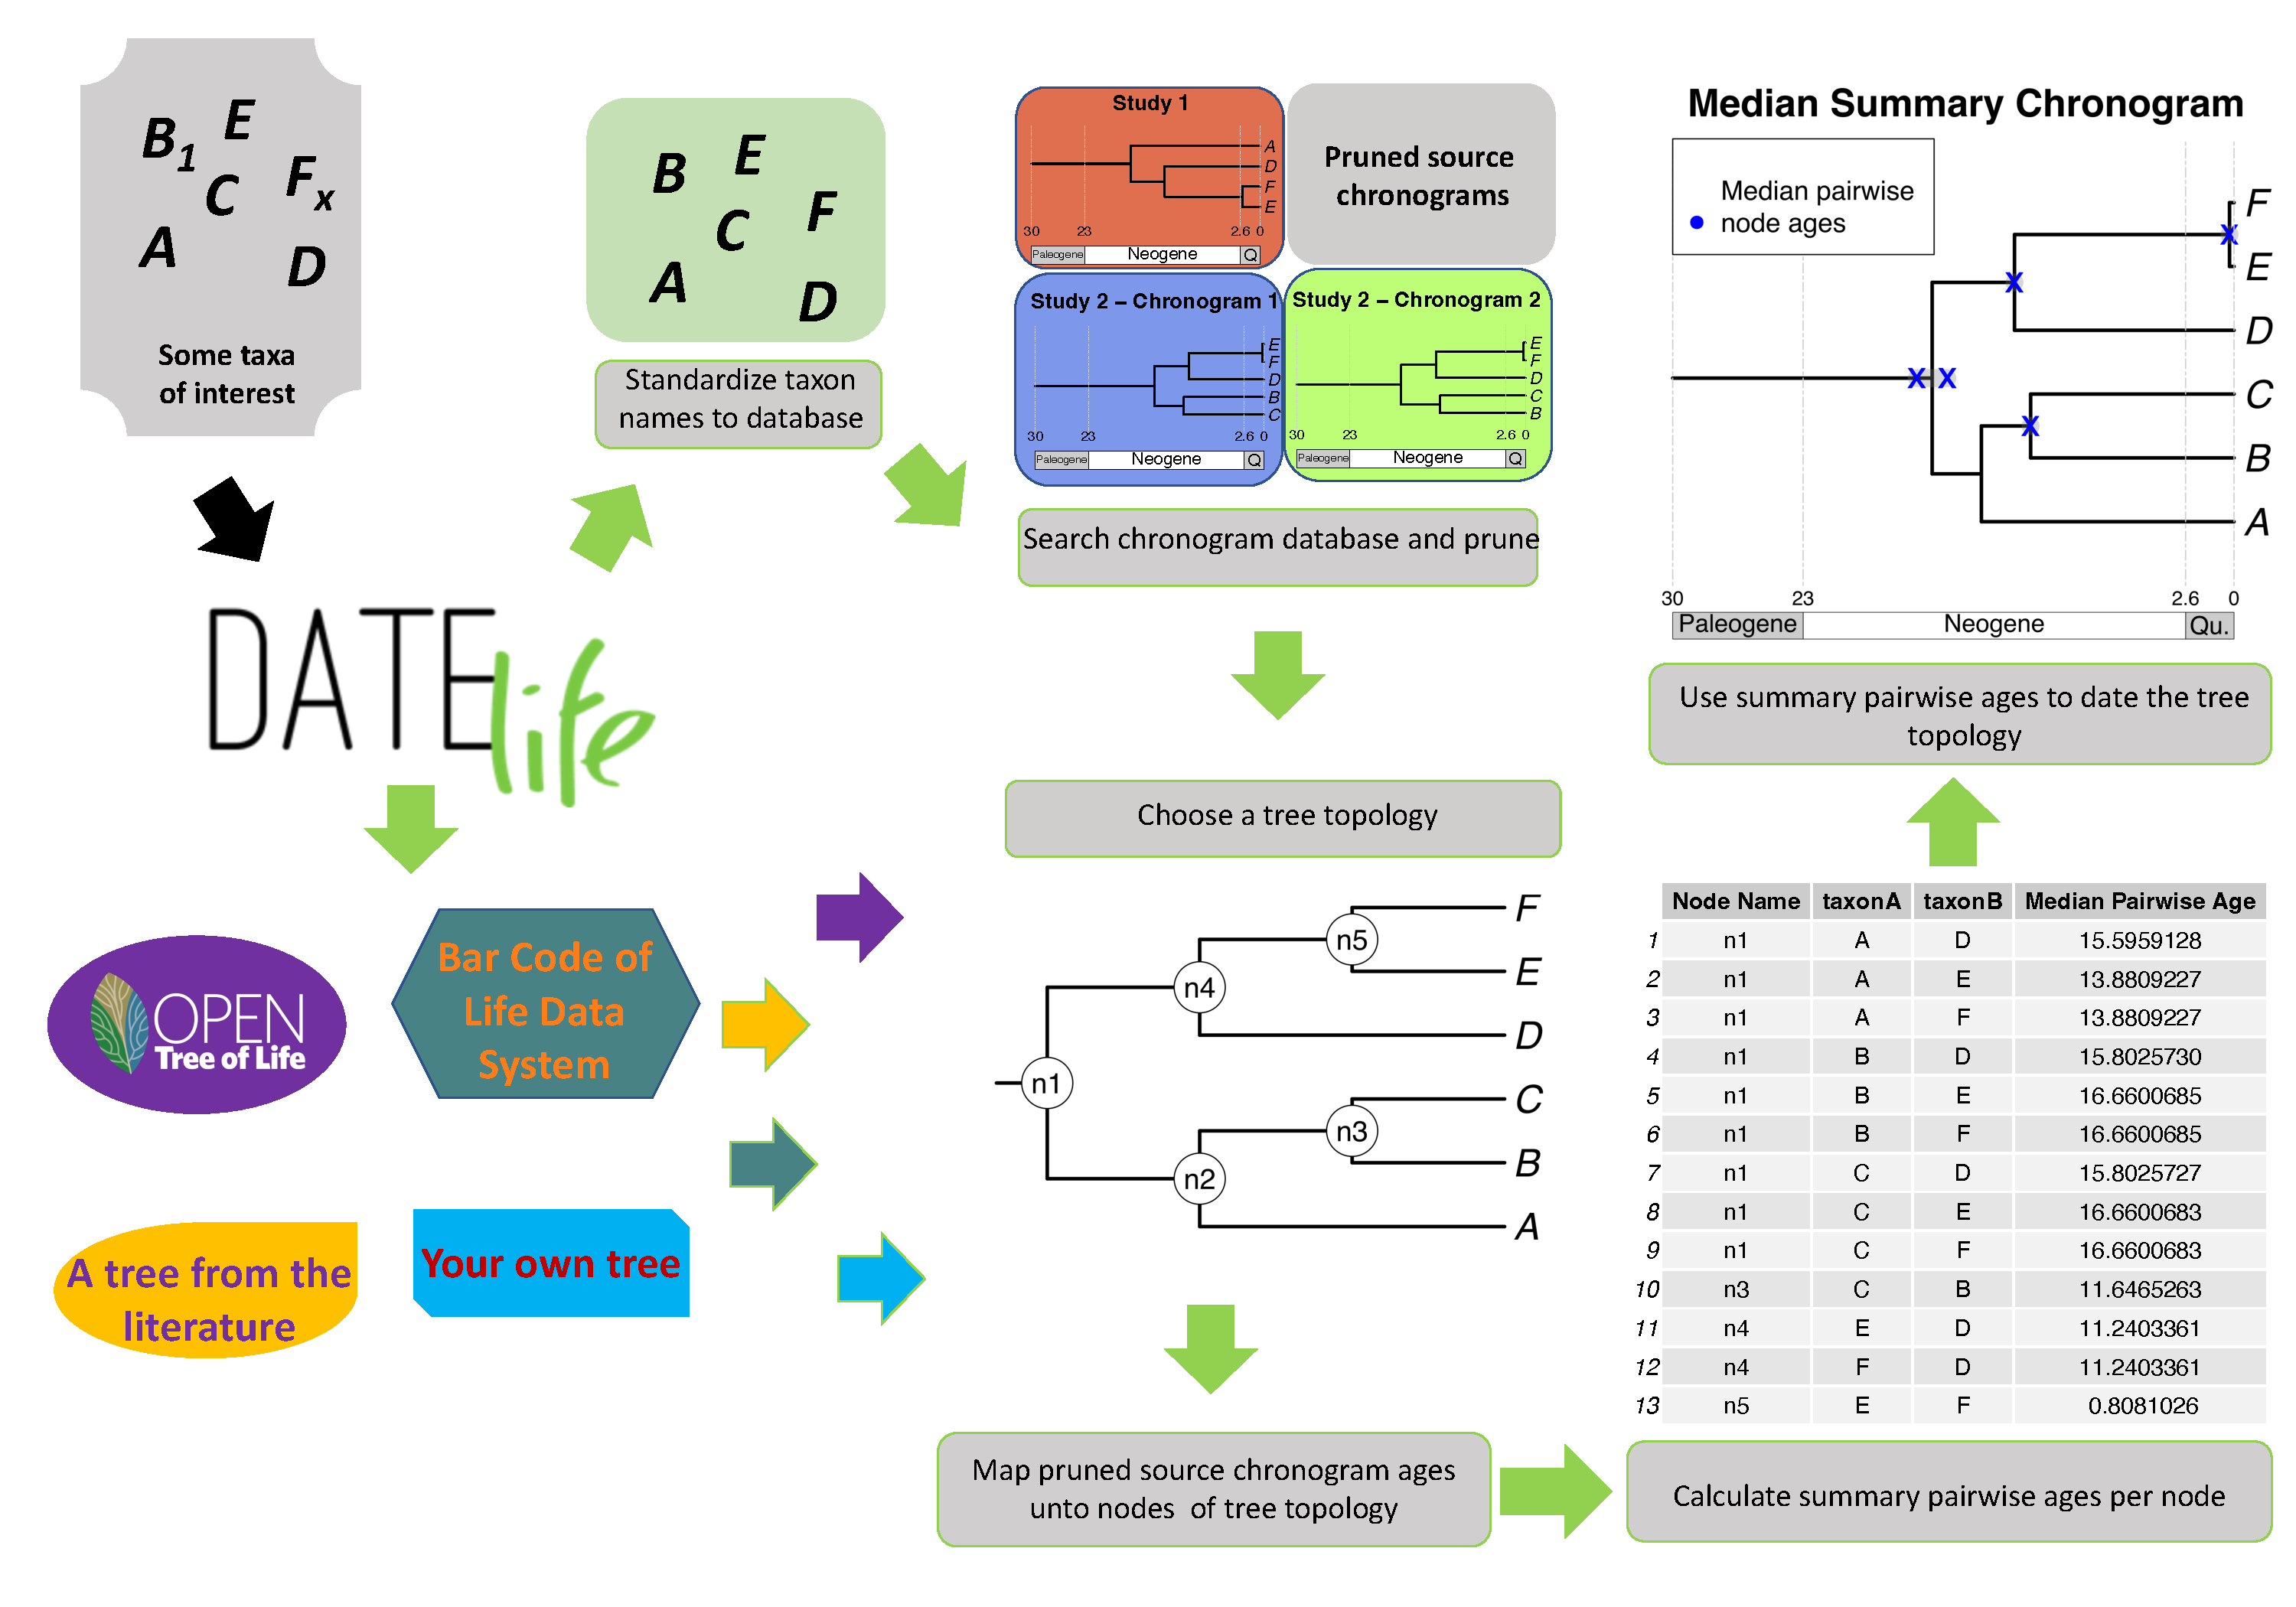
\includegraphics{../figures/figure1/figure1-vertical-final.pdf}
\caption{
Stylized DateLife algorithm showing the main steps that are performed
with the R package \texttt{datelife}, or online at \url{www.datelife.org/query/}.
Details on the functions involved on each workflow are available at \texttt{datelife}'s
R package manual https://phylotastic.org/datelife/articles/.
}
\label{fig:workflow}
\end{figure}

%%%%%%%%%%%%%%%%%%%%%%%%%%%%%%%%%%%%%%%%%%%%%%%%%%%%%%%%%%%%%%%%%%%%%%%%%%%%%%%%
%%%%%%%%%%%%%%%%%%%%%%%%%%%%%%%%%%%%%%%%%%%%%%%%%%%%%%%%%%%%%%%%%%%%%%%%%%%%%%%%
%% BENCHMARK FIGURE
%%%%%%%%%%%%%%%%%%%%%%%%%%%%%%%%%%%%%%%%%%%%%%%%%%%%%%%%%%%%%%%%%%%%%%%%%%%%%%%%
%%%%%%%%%%%%%%%%%%%%%%%%%%%%%%%%%%%%%%%%%%%%%%%%%%%%%%%%%%%%%%%%%%%%%%%%%%%%%%%%
\newpage
\begin{figure}[!h]
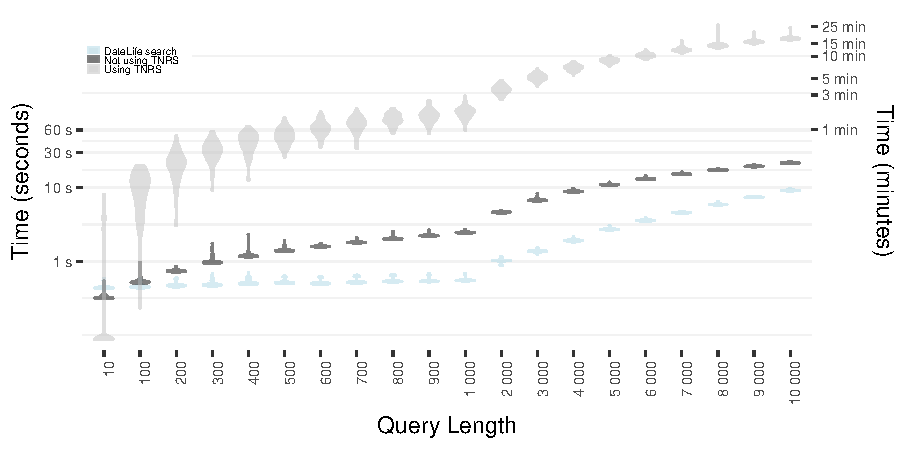
\includegraphics{../figures/fig_runtime_main.pdf}
\caption{Input taxon name processing and chronogram database search computation time increases with number of input taxon names. We sampled N bird species names for each input size class, 100 times, and then performed a \texttt{datelife} search using the Taxon Names Resoultion Service (TNRS; light gray), and without using TNRS (dark gray). We also performed a search using the already processed query for comparison (light blue).}
\label{fig:benchmark}
\end{figure}
\newpage

%%%%%%%%%%%%%%%%%%%%%%%%%%%%%%%%%%%%%%%%%%%%%%%%%%%%%%%%%%%%%%%%%%%%%%%%%%%%%%%%
%%%%%%%%%%%%%%%%%%%%%%%%%%%%%%%%%%%%%%%%%%%%%%%%%%%%%%%%%%%%%%%%%%%%%%%%%%%%%%%%
%% SMALL EXAMPLE FIGURES
%%%%%%%%%%%%%%%%%%%%%%%%%%%%%%%%%%%%%%%%%%%%%%%%%%%%%%%%%%%%%%%%%%%%%%%%%%%%%%%%
%%%%%%%%%%%%%%%%%%%%%%%%%%%%%%%%%%%%%%%%%%%%%%%%%%%%%%%%%%%%%%%%%%%%%%%%%%%%%%%%

\newpage
\begin{figure}[!h]
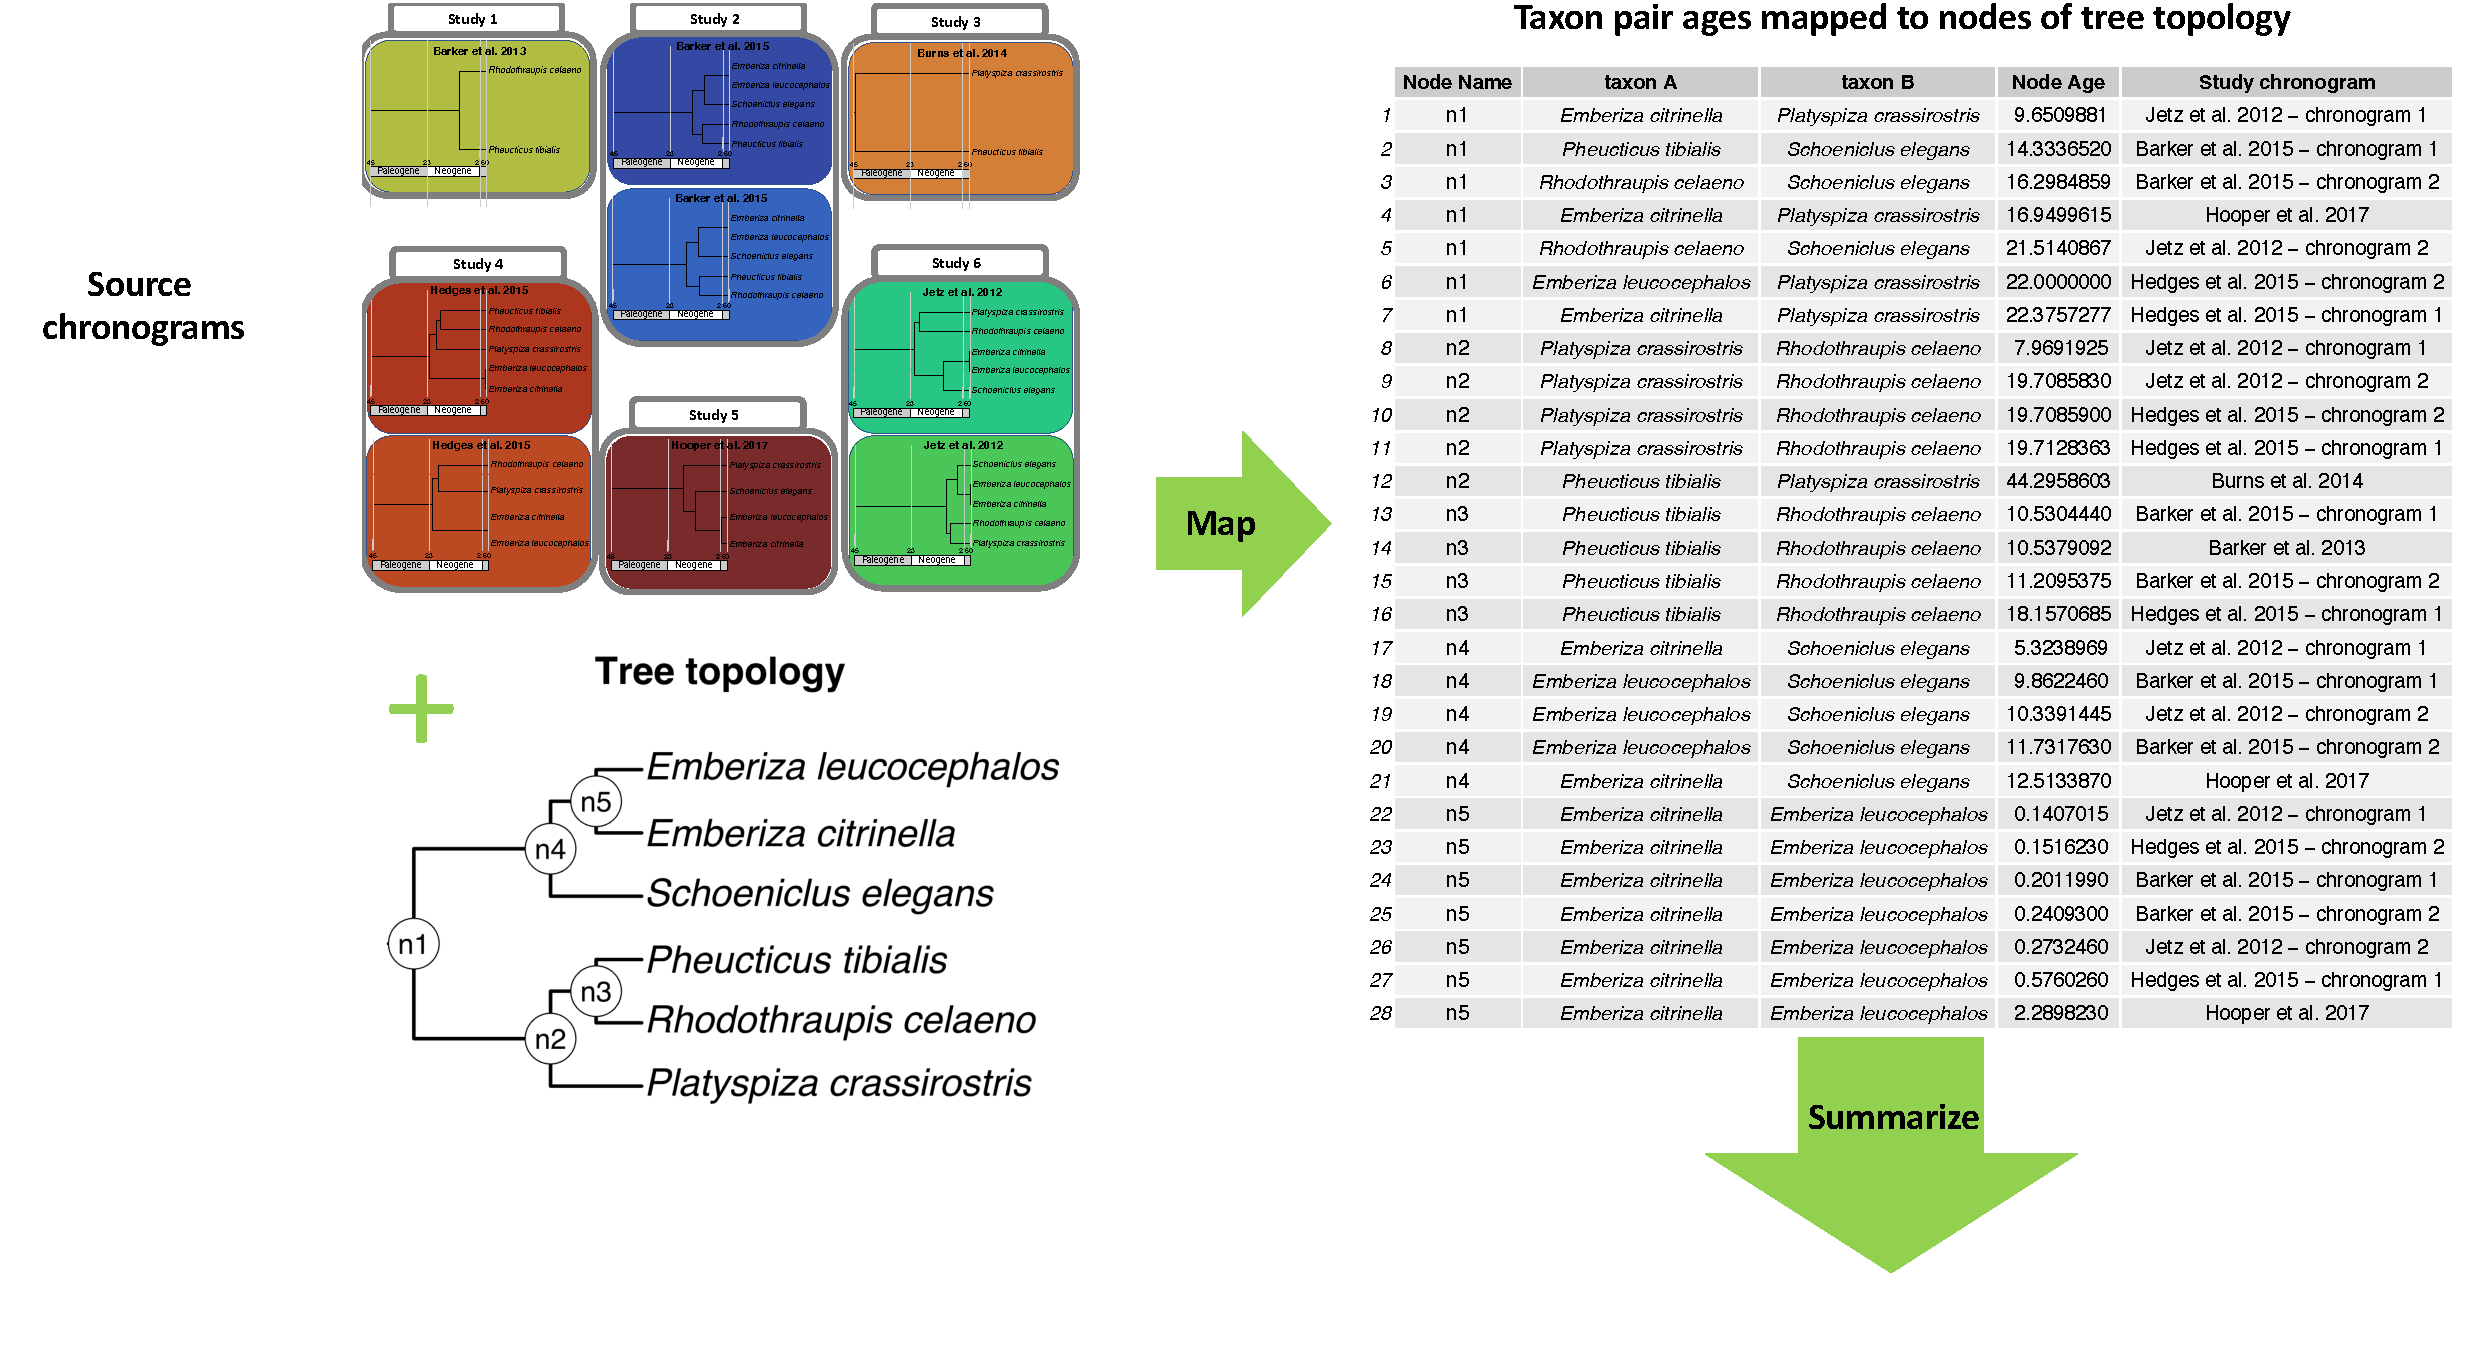
\includegraphics[width=1\linewidth]{../figures/figure2/figure2-1.pdf}
\caption{
Age data results of a DateLife search of a small sample of 6 bird species within the Passeriformes. Input names were found across 9 chronograms within 6 independent studies (Barker et al. (\protect\hyperlink{ref-barker2012going}{2012}), Barker et al. (\protect\hyperlink{ref-barker2015new}{2015}), Burns et al. (\protect\hyperlink{ref-burns2014phylogenetics}{2014}), Hedges et al. (\protect\hyperlink{ref-Hedges2015}{2015}), Hooper and Price (\protect\hyperlink{ref-hooper2017chromosomal}{2017}), Jetz et al. (\protect\hyperlink{ref-Jetz2012}{2012}).) This revealed 28 age data points for the queried species names.
}
\label{fig:figure2-1}
\end{figure}

\newpage
\begin{figure}[!h]
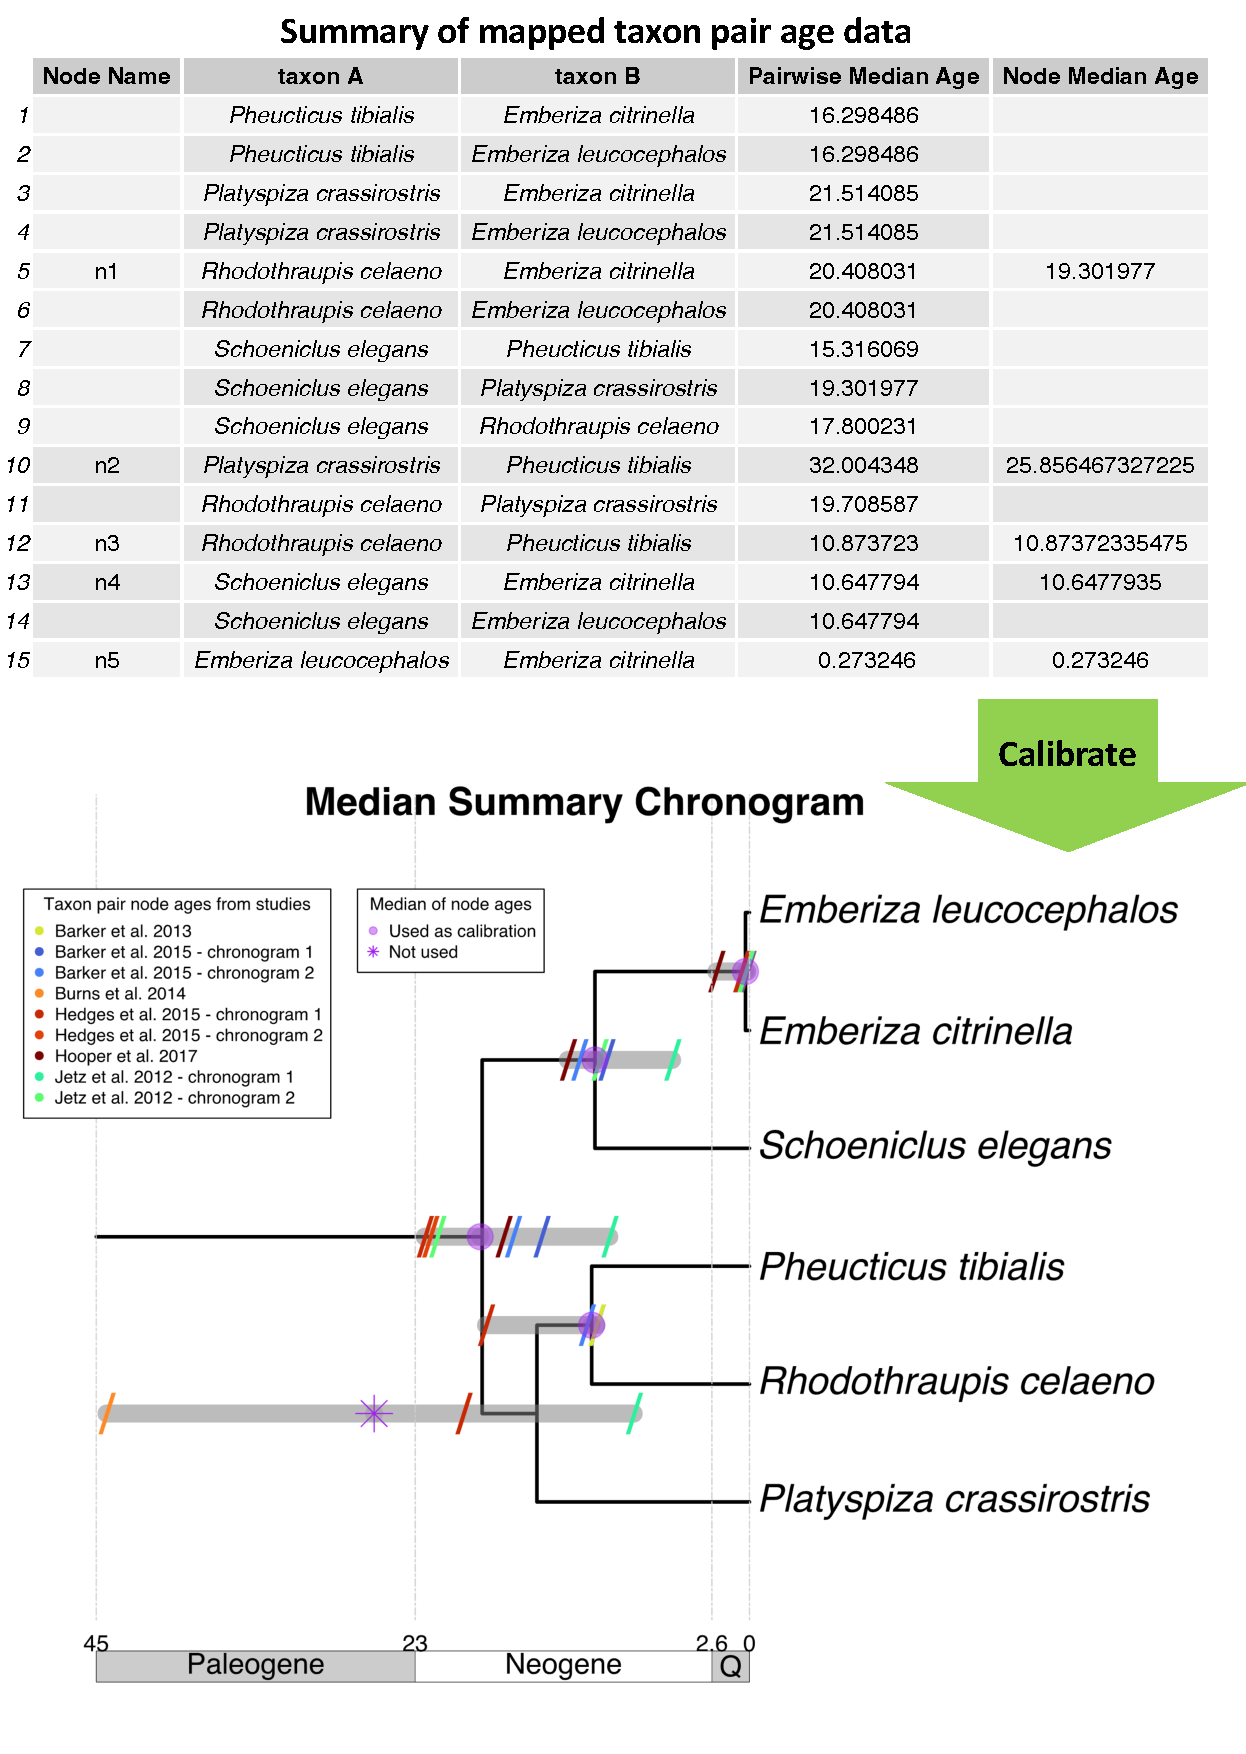
\includegraphics[width=1\linewidth]{../figures/figure2/figure2-2.pdf}
\caption{
Summarized age data is used as secondary calibrations to obtain a summary chronogram.
}
\label{fig:figure2-2}
\end{figure}

%%%%%%%%%%%%%%%%%%%%%%%%%%%%%%%%%%%%%%%%%%%%%%%%%%%%%%%%%%%%%%%%%%%%%%%%%%%%%%%%
%%%%%%%%%%%%%%%%%%%%%%%%%%%%%%%%%%%%%%%%%%%%%%%%%%%%%%%%%%%%%%%%%%%%%%%%%%%%%%%%
%% REAL LIFE APP FIGURE
%%%%%%%%%%%%%%%%%%%%%%%%%%%%%%%%%%%%%%%%%%%%%%%%%%%%%%%%%%%%%%%%%%%%%%%%%%%%%%%%
%%%%%%%%%%%%%%%%%%%%%%%%%%%%%%%%%%%%%%%%%%%%%%%%%%%%%%%%%%%%%%%%%%%%%%%%%%%%%%%%

\newpage
\begin{figure}[!h]
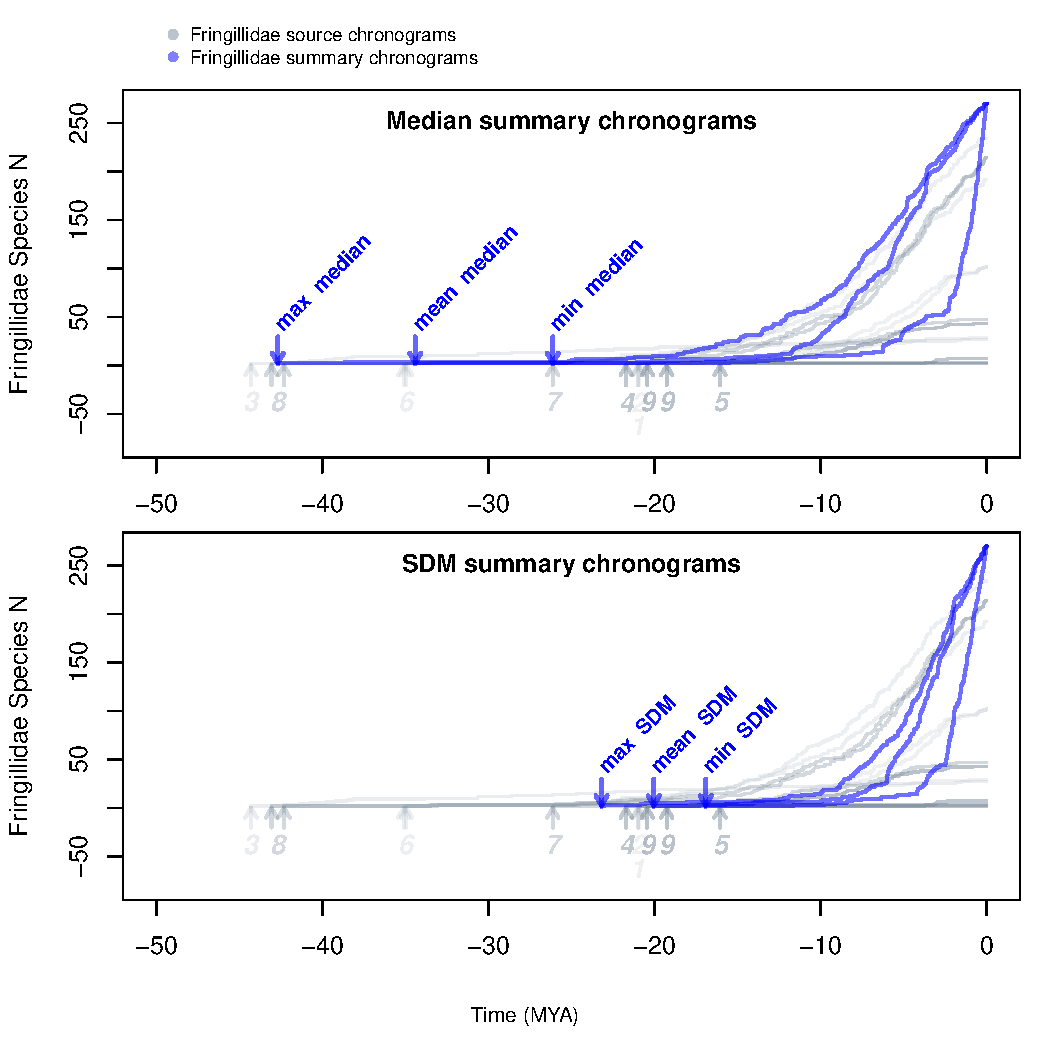
\includegraphics{../figures/fig_summaries.pdf}
\caption{LTT plots of median (top) and Supermatrix Distance Method (SDM; bottom) chronograms summarising information from source chronograms found for the Fringillidae. Arrows indicate tree maximum age.}
\label{fig:summaries}
\end{figure}

%%%%%%%%%%%%%%%%%%%%%%%%%%%%%%%%%%%%%%%%%%%%%%%%%%%%%%%%%%%%%%%%%%%%%%%%%%%%%%%%
%%%%%%%%%%%%%%%%%%%%%%%%%%%%%%%%%%%%%%%%%%%%%%%%%%%%%%%%%%%%%%%%%%%%%%%%%%%%%%%%
%% CROSS VALIDATION FIGURES
%%%%%%%%%%%%%%%%%%%%%%%%%%%%%%%%%%%%%%%%%%%%%%%%%%%%%%%%%%%%%%%%%%%%%%%%%%%%%%%%
%%%%%%%%%%%%%%%%%%%%%%%%%%%%%%%%%%%%%%%%%%%%%%%%%%%%%%%%%%%%%%%%%%%%%%%%%%%%%%%%

\newpage
\begin{figure}[!h]
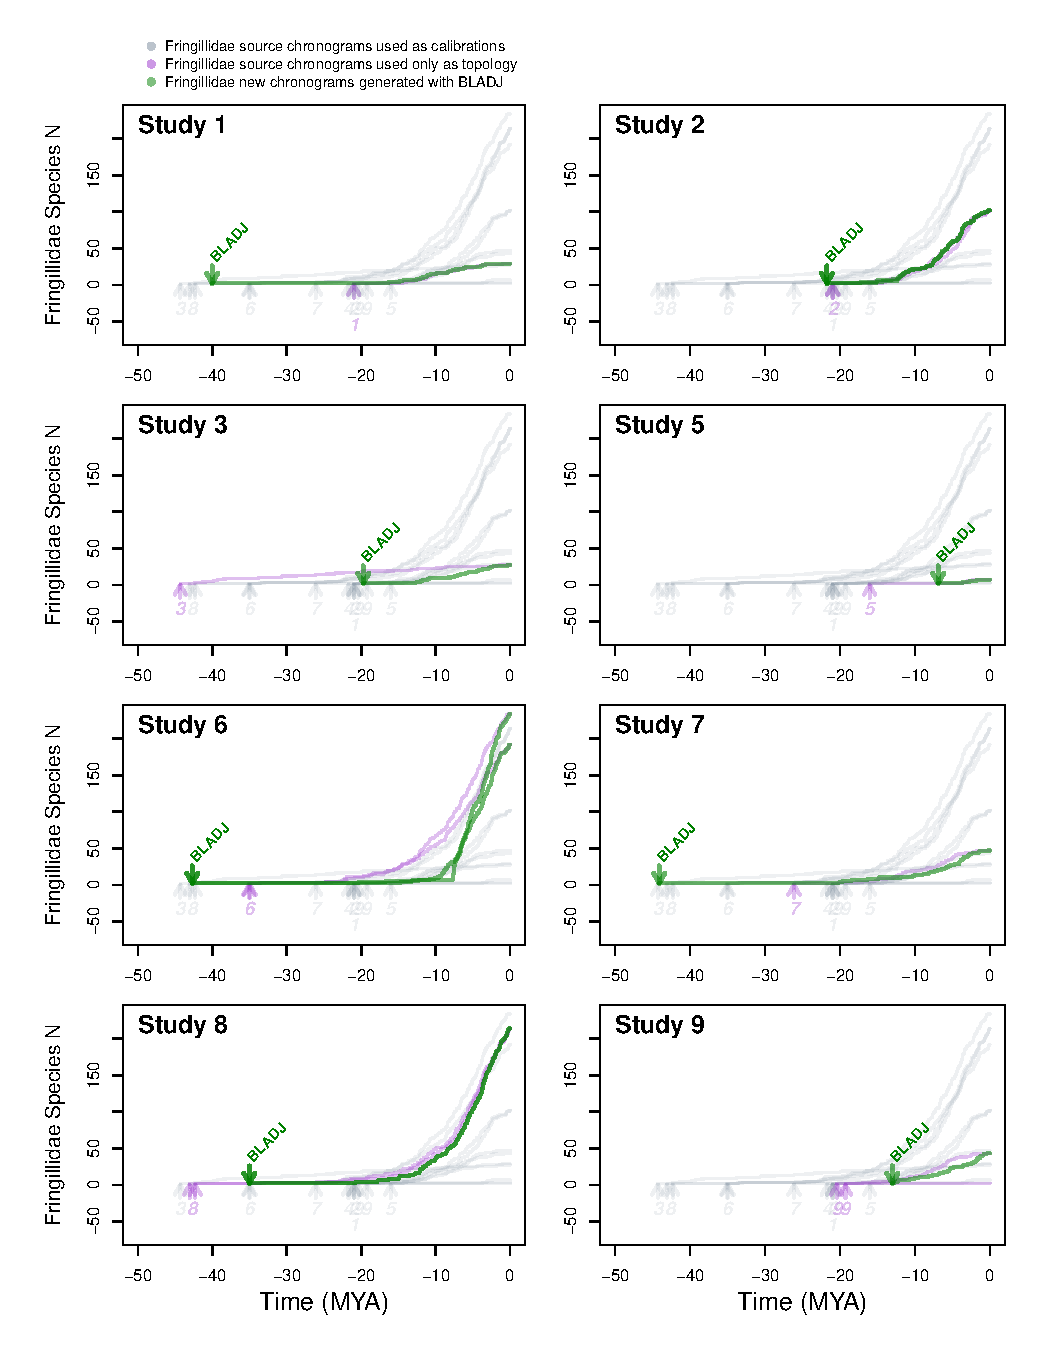
\includegraphics{../figures/fig_crossval_bladj.pdf}
\caption{LTT plots showing results from the cross-validation analyses of trees without branch lengths dated using BLADJ. The dating analysis can only be performed in trees with more than 2 tips, thus excluding chronogram from study 4; its data was still used as calibration for the other source chronograms.}
\label{fig:cvbladj}
\end{figure}

\newpage
\begin{figure}[!h]
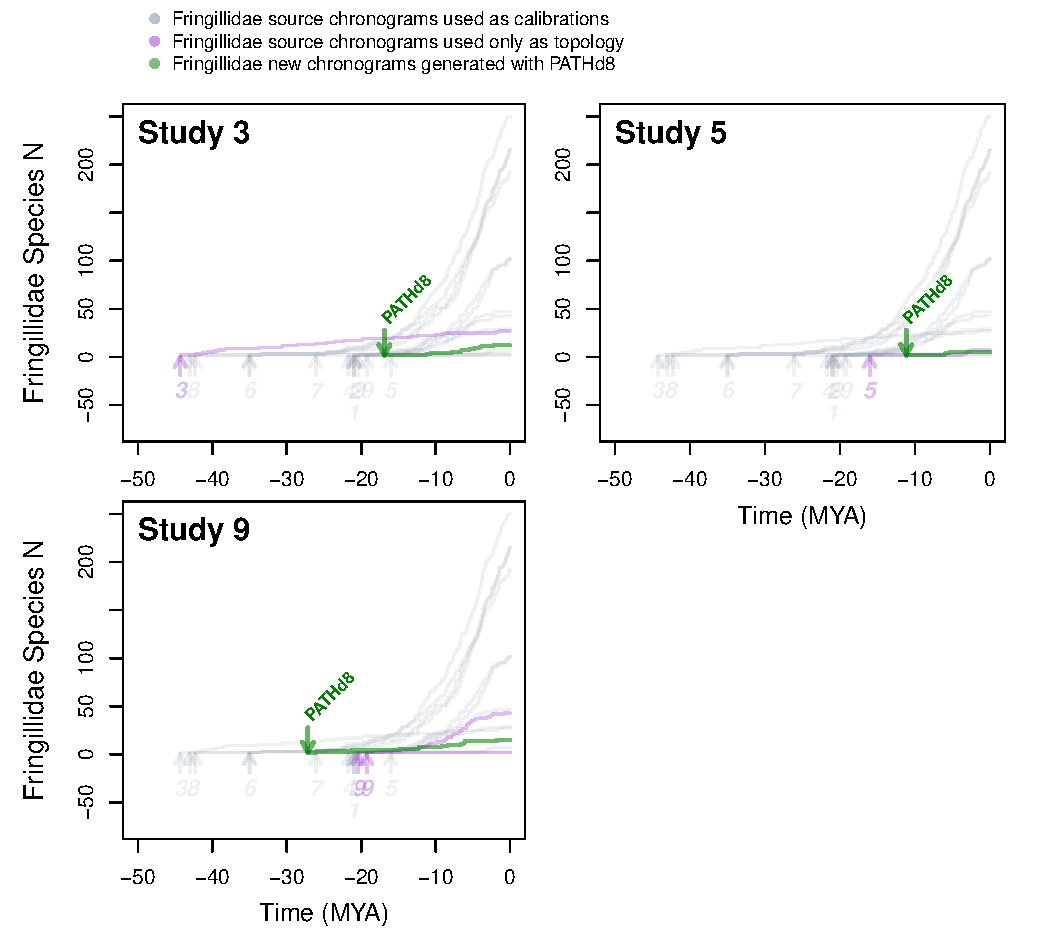
\includegraphics{../figures/fig_crossval_boldsumm.pdf}
\caption{LTT plots showing results from the cross-validation analyses of trees with branch length reconstructed with data from the Barcode of Life Database (BOLD) dated using PATHd8. We could construct a tree with branch lengths for all source chronograms. However, dating with PATHd8 was only successful in three source chronograms shown here.}
\label{fig:cvbold}
\end{figure}
